% Labelling -- anatomical labelling of the airway trees with the released IPGN model.
% Red \TODO{...} marks replace the [square-bracket] placeholders of the original draft.

\section[Labelling]{Anatomical Labeling of Airway Trees}
\label{sec:labeling}                     % \secref{sec:labeling}

To assign anatomical labels to our airway trees, we used the Implicit Point-Graph Network
(IPGN) of \citet{xie2025}. We did not train this model ourselves: we used the weights
released by the authors, trained on their Pulmonary Tree Labeling (PTL) dataset, and ran the
model in inference mode only. This section describes how the model is formulated and how it
was trained, so that its predictions on our data can be interpreted.

% ------------------------------------------------------------------------------
\subsection{Task formulation}            % 19-class labeling of a binary tree
\label{sec:labeling_task}                % \secref{sec:labeling_task}

The input to the model is a binary volume containing a pulmonary tree (airway, artery or
vein). The goal is a 19-class semantic segmentation of every foreground voxel: 18 classes
correspond to segmental-level branches, i.e.\ the branches that supply the 18 pulmonary
segments, and one class corresponds to the extra-pulmonary structures \cite{xie2025}. Labels
1 to 10 are branches in the left lung, labels 11 to 18 are branches in the right lung, and
label 19 is the extra-pulmonary part (for the airway, the trachea and main
bronchi) \cite{xie2025}.

Xie et al.\ point out that the hardest part of this task is labeling the branching points and
the distal end points correctly. These key locations contain very few voxels compared to the
rest of the tree, so a model trained only on voxel-wise signals is dominated by easy voxels
and can achieve a high voxel-level score while still mislabeling key
locations \cite{xie2025}. For this reason, IPGN also represents each tree as a skeleton graph
whose nodes approximate these key points, and it is evaluated on both voxels and graph
elements.

% ------------------------------------------------------------------------------
\subsection{Training data}               % PTL dataset and skeleton graph labels
\label{sec:labeling_data}                % \secref{sec:labeling_data}

\paragraph{PTL dataset.}                 % the data the released model was trained on
The model was trained on the PTL dataset, compiled by the authors from multiple medical
centers \cite{xie2025}. It contains 800 subjects, each with three volumes (airway, artery and
vein) annotated with the 19 classes above. All volumes have size $N \times 512 \times 512$,
with $N$ between 181 and 798 slices and a slice spacing between 0.5 and 1.5~mm. The
annotations were produced by a junior radiologist and verified by a senior radiologist.
During training, each annotated volume is converted to a binary input, and the original
labeled volume is the prediction target. The dataset was split randomly into 70\% training,
10\% validation and 20\% test subjects \cite{xie2025}.

\paragraph{Skeleton graphs.}             % how graphs are built from volumes
For each volume, a skeleton graph is built with the VesselVio software \cite{bumgarner2022},
which applies the thinning algorithm of \citet{lee1994} to extract the centerlines of the
tree. In the resulting graph, the centerline segments become edges representing anatomical
connections, and the centerline intersections and distal end points become nodes
representing the key points of the tree \cite{xie2025}. No additional hyperparameters or
modeling are involved: all spatial and connectivity information comes directly from the
original volume.

\paragraph{Graph labels.}                % three-step labeling procedure
Ground-truth labels for the graph are derived from the annotated volume in three steps,
labeling edges before nodes because edge labels are deterministic while node labels can be
ambiguous where classes meet \cite{xie2025}:
\begin{enumerate}                        % the graph labeling procedure
  \item \textbf{Graph simplification.} VesselVio also outputs, for each edge, the connected
        centerline points along it. Software inconsistencies can create cliques among
        these points; they are removed by keeping only the shortest path between the two
        nodes.
  \item \textbf{Edge labeling.} The labels of the centerline points of each edge are read
        from the annotated volume, and the edge label is their majority vote.
  \item \textbf{Node labeling.} A leaf node takes the label of its single edge, which is
        more reliable than reading it from the volume, since leaf coordinates can fall
        slightly outside the foreground. A node with several edges takes the majority vote
        of the labels of its connected edges.
\end{enumerate}

% ------------------------------------------------------------------------------
\subsection{Model architecture}          % PGN backbone + Implicit Point Module
\label{sec:labeling_architecture}        % \secref{sec:labeling_architecture}

\paragraph{Overview.}                    % the three stages of IPGN
Instead of processing the dense volume with a CNN, IPGN works on two sparse representations
of the tree: a point cloud, obtained by randomly sampling $M = 6{,}000$ foreground voxels,
and the skeleton graph with $N$ nodes \cite{xie2025}. The point cloud is a downsampled
version of the volume, while the graph describes the skeleton of the tree. The model has three
stages (Figure~\ref{fig:ipgn_overview}): separate point and graph encoders, a sequence of
Point-Graph Fusion layers that exchange information between the two branches, and an
Implicit Point Module that turns the sparse predictions back into a dense labeled volume. The
network without the implicit part is called the Point-Graph Network (PGN), and the full
model is IPGN \cite{xie2025}.

\paragraph{Notation.}                    % points, nodes and layer features
The point coordinates are $\mathbf{P} = \{\mathbf{p}_1, \dots, \mathbf{p}_M\} \in
\mathbb{R}^{M\times3}$ and the graph node coordinates are $\mathbf{G} = \{\mathbf{g}_1,
\dots, \mathbf{g}_N\} \in \mathbb{R}^{N\times3}$. A superscript $(i)$ denotes the feature of
an element after the $i$-th layer, e.g.\ $\mathbf{p}^{(i)}$ and $\mathbf{g}^{(i)}$, and
$\frown$ denotes concatenation \cite{xie2025}.

\paragraph{Point and graph encoders.}    % initial per-element features
The $(x, y, z)$ coordinates of the points and of the graph nodes are the only input features.
A point network and a graph network act as initial encoders and produce a 128-dimensional
feature for each point and each node, $\mathbf{P}^{(0)} \in \mathbb{R}^{M\times128}$ and
$\mathbf{G}^{(0)} \in \mathbb{R}^{N\times128}$ \cite{xie2025}. The point encoder is either
PointNet++ \cite{qi2017} or Point Transformer \cite{zhao2021}, and the graph encoder is an
11-layer graph attention network (GAT) \cite{velickovic2018} with 128 channels. The model we
used has a \TODO{PointNet++ / Point Transformer} point encoder.

\paragraph{Point-Graph Fusion layers.}   % two-way feature exchange
The core of the model is a stack of $l$ Point-Graph Fusion layers
(Figure~\ref{fig:ipgn_fusion}). Each layer takes $\mathbf{P}^{(i-1)}$ and
$\mathbf{G}^{(i-1)}$ and outputs $\mathbf{P}^{(i)}$ and $\mathbf{G}^{(i)}$, using the 3D
coordinates of the elements to find neighbors in the other branch \cite{xie2025}.

\emph{Point to graph (ball query and grouping).} Each graph node $\mathbf{g}$ collects all
points within a ball of radius $r$ around it, $\{\mathbf{p}_1, \dots, \mathbf{p}_b\}$, in
the style of PointNet++ \cite{qi2017}. An MLP $\mathcal{F}_1$ updates each of these point
features independently, and feature-wise max pooling aggregates them into a point summary
for the node \cite{xie2025}:
\begin{equation}
  \mathbf{g}^{(i)}_{bq} = \max_{j}\, \mathcal{F}_1\big(\mathbf{p}^{(i-1)}_j\big).
  \label{eq:ipgn_bq}                     % ball query + max pooling
\end{equation}
This summary is concatenated with the current node feature and passed through a shallow
graph attention network $\mathcal{G}$ \cite{velickovic2018}, which performs graph
convolution to produce the updated node feature:
\begin{equation}
  \mathbf{g}^{(i)} = \mathcal{G}\big(\mathbf{g}^{(i-1)} \frown \mathbf{g}^{(i)}_{bq}\big),
  \qquad \mathcal{G}: \mathbb{R}^{2D} \to \mathbb{R}^{D_{\mathrm{next}}}.
  \label{eq:ipgn_gat}                    % graph update with GAT
\end{equation}

\emph{Graph to point (feature propagation).} Each point $\mathbf{p}$ finds its $k$ nearest
graph nodes $\{\mathbf{g}_1, \dots, \mathbf{g}_k\}$ in coordinate space, at distances
$\{d_1, \dots, d_k\}$, and combines their features with weights given by the normalized
inverse distances \cite{rossi2021,xie2025}:
\begin{equation}
  \mathbf{p}^{(i)}_{fp} = \frac{\sum_{j=1}^{k} \mathbf{g}^{(i-1)}_j \cdot \frac{1}{d_j}}
                               {\sum_{l=1}^{k} \frac{1}{d_l}}.
  \label{eq:ipgn_fp}                     % inverse-distance feature propagation
\end{equation}
The result is concatenated with the incoming point feature, and an MLP $\mathcal{F}_2$
projects it to the next layer's dimension:
\begin{equation}
  \mathbf{p}^{(i)} = \mathcal{F}_2\big(\mathbf{p}^{(i-1)} \frown \mathbf{p}^{(i)}_{fp}\big),
  \qquad \mathcal{F}_2: \mathbb{R}^{2D} \to \mathbb{R}^{D_{\mathrm{next}}}.
  \label{eq:ipgn_mlp}                    % point update with MLP
\end{equation}
In this way, the points receive the structural context of the skeleton, and the graph
receives the local shape information of the surrounding points. After the last fusion
layer, a lightweight MLP and a GNN project the point and node features to 19-dimensional
class scores \cite{xie2025}.

\paragraph{Implicit Point Module.}       % sparse-to-dense reconstruction
PGN only labels the 6,000 sampled points and the graph nodes. Labeling every foreground voxel
by repeatedly running PGN on new point clouds would be inefficient, because the graph and the
global shape of the point cloud do not change between runs \cite{xie2025}. The Implicit Point
Module instead treats the point features learned by PGN as a continuous feature field that
can be queried at any location (Figure~\ref{fig:ipgn_overview}). For a query point
$\mathbf{p}_q = (x_q, y_q, z_q)$, which does not need to belong to the sampled point cloud:
\begin{enumerate}                        % the three steps of the implicit module
  \item its $k$ nearest neighbors $\{\mathbf{p}_1, \dots, \mathbf{p}_k\}$ in the sampled
        point cloud are found;
  \item for each neighbor, its features from all stages of PGN are concatenated into a
        multi-stage feature
        $\mathbf{z}_k = \mathbf{p}^{(0)}_k \frown \mathbf{p}^{(1)}_k \frown \dots \frown
        \mathbf{p}^{(l)}_k$, and these are combined into a feature $\mathbf{z}_q$ for the
        query point by inverse-distance feature propagation, as in
        Equation~\eqref{eq:ipgn_fp};
  \item an MLP $\mathcal{H}$ maps $\mathbf{z}_q$ to a 19-dimensional vector of class
        scores \cite{xie2025}.
\end{enumerate}
Using features from all stages, rather than only the last fusion layer, gave the best
results in the authors' ablation study \cite{xie2025}.

\paragraph{Hyperparameters.}             % values reported by the authors
The ball query uses a radius $r = 0.1$ and at most 24 points per node; $\mathcal{G}$ is a
3-layer GAT; the $k$-nearest-neighbor search in both the graph-to-point fusion and the
Implicit Point Module uses $k = 3$; and all intermediate fusion features are
128-dimensional \cite{xie2025}. With a PointNet++ encoder, PGN has about 3.6M parameters,
and the Implicit Point Module adds about 0.1M \cite{xie2025}.

\begin{figure}[htbp]                     % placeholder for the IPGN overview figure
  \centering                             % center the figure
  % 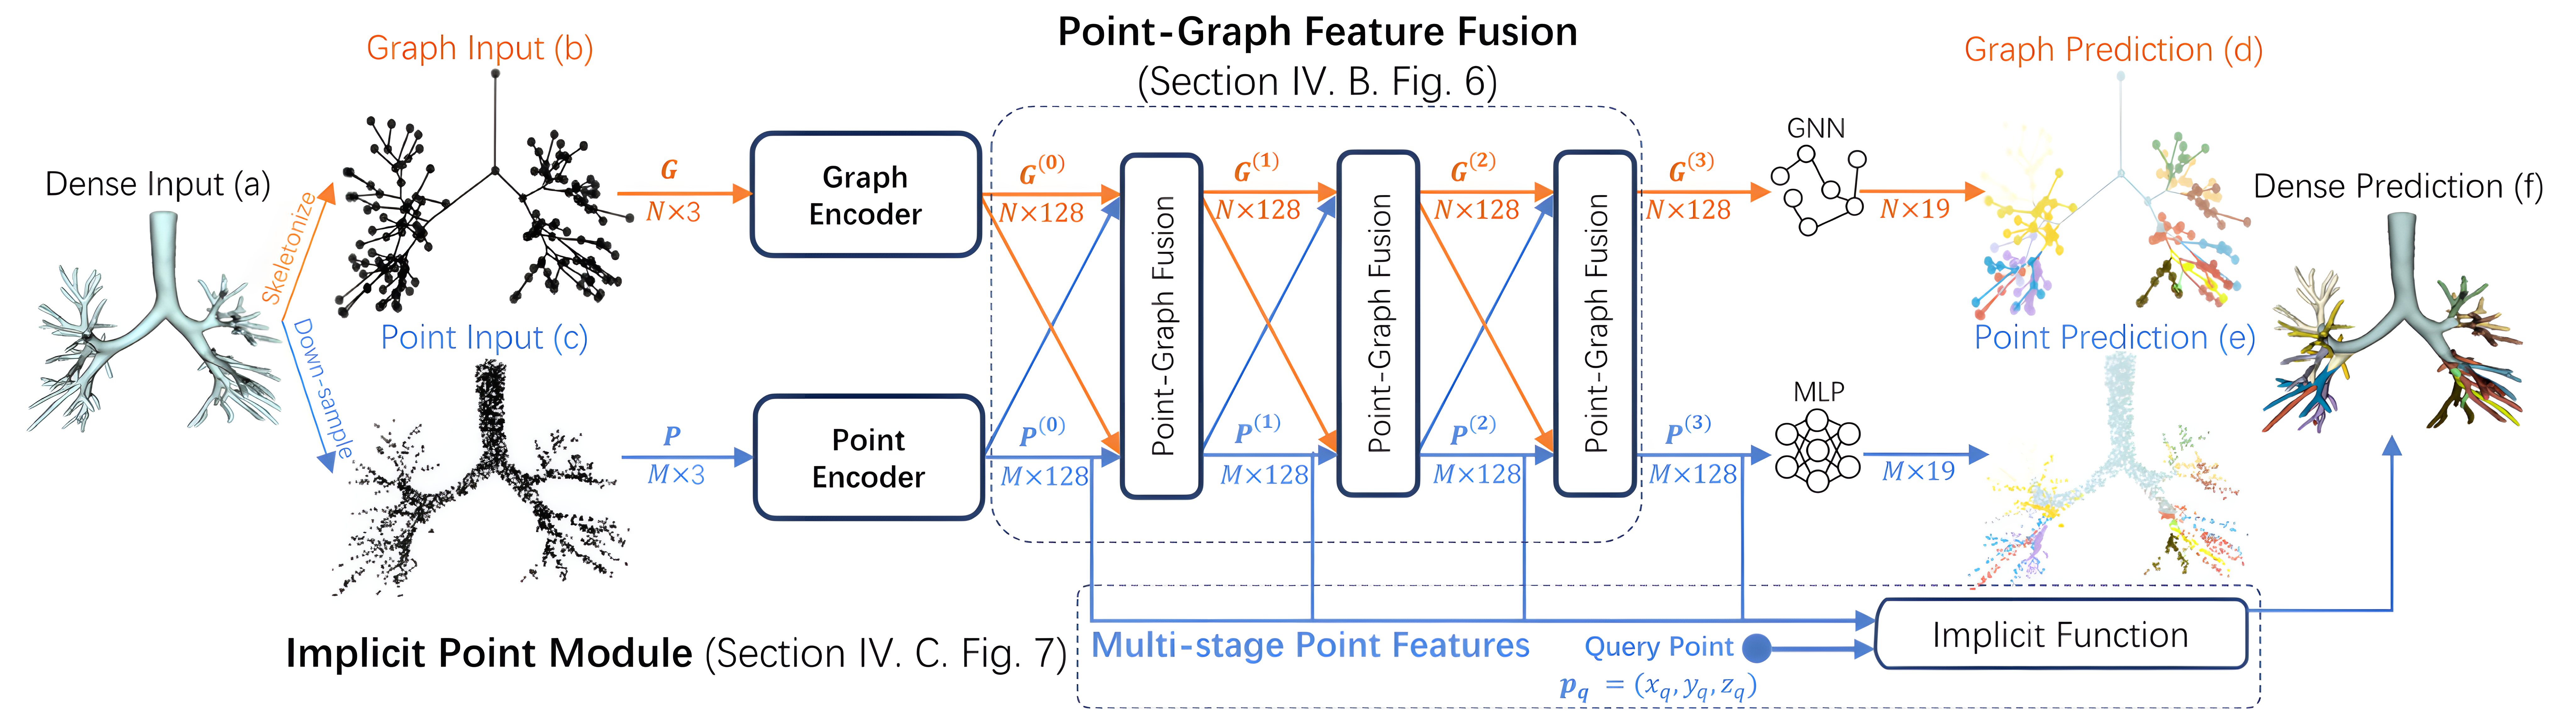
\includegraphics[width=\textwidth]{figures/ipgn_overview.png}  % uncomment with your file
  \fbox{\parbox[c][4cm][c]{0.9\textwidth}{\centering [IPGN overview figure]}}  % remove once image added
  \caption{Overview of the Implicit Point-Graph Network (IPGN), adapted from
           \citet{xie2025}. The binary volume is converted into a skeleton graph and a
           point cloud, Point-Graph Fusion layers exchange features between the two
           branches, and the Implicit Point Module produces the dense labeled volume.}
  \label{fig:ipgn_overview}              % referenced as Figure~\ref{fig:ipgn_overview}
\end{figure}

\begin{figure}[htbp]                     % placeholder for the fusion-layer figure
  \centering                             % center the figure
  % \includegraphics[width=\textwidth]{figures/ipgn_fusion_layer.png}  % uncomment with your file
  \fbox{\parbox[c][4cm][c]{0.9\textwidth}{\centering [Point-Graph Fusion layer figure]}}  % remove once image added
  \caption{A Point-Graph Fusion layer, adapted from \citet{xie2025}. Graph nodes gather point
           features by ball query and grouping; points gather graph features by
           $k$-nearest-neighbor feature propagation.}
  \label{fig:ipgn_fusion}                % referenced as Figure~\ref{fig:ipgn_fusion}
\end{figure}

% ------------------------------------------------------------------------------
\subsection{Training}                    % how the released weights were obtained
\label{sec:labeling_training}            % \secref{sec:labeling_training}

The released model was trained by Xie et al.\ in two stages \cite{xie2025}.

\paragraph{Encoder pre-training.}        % encoders trained separately and frozen
First, the point encoder and the graph encoder were trained independently on the point and
graph versions of the 19-class labeling task, and then frozen. The point encoders were
trained for 120 epochs with a learning rate of 0.002, and the GAT graph encoder for 240
epochs with a learning rate of 0.02 \cite{xie2025}.

\paragraph{Joint training.}              % PGN + implicit module trained together
Second, PGN and the Implicit Point Module were trained together. In each step, PGN is run on
$M = 6{,}000$ sampled points and the $N$ graph nodes, producing multi-stage features and
predictions for all of them. A second, independent set of $M' = 6{,}000$ foreground points
is then sampled and passed through the Implicit Point Module as query points. The
cross-entropy loss is applied to all $M + M'$ point predictions and all $N$ graph
predictions \cite{xie2025}. This stage ran for 100 epochs with a learning rate of 0.01,
halved every 45 epochs. Random rotation, shifting and scaling were used as data augmentation
to avoid overfitting \cite{xie2025}.

% ------------------------------------------------------------------------------
\subsection{Inference}                   % how the labels on our trees are produced
\label{sec:labeling_inference}           % \secref{sec:labeling_inference}

Inference follows the procedure of \citet{xie2025}:
\begin{enumerate}                        % the inference steps
  \item \textbf{Pre-processing.} The binary airway volume is skeletonized to obtain the
        skeleton graph (\secref{sec:labeling_data}), and 6,000 foreground voxels are
        randomly sampled as the point cloud.
  \item \textbf{Point-Graph Network.} A single forward pass of PGN on the graph and point
        cloud gives the multi-stage point features and the labels of the graph nodes.
  \item \textbf{Dense labeling.} All remaining foreground voxels are grouped into batches
        and passed through the Implicit Point Module as query points, which gives a label
        for every voxel of the tree.
\end{enumerate}
Because PGN only runs once, dense labeling is fast: the authors report around 1.3~s per
airway tree with a PointNet++ encoder and 2.3~s with Point Transformer, against 5.7~s and
12.1~s when PGN is run repeatedly over the whole volume \cite{xie2025}.

% ------------------------------------------------------------------------------
\subsection{Reported performance}        % metrics and results from the paper
\label{sec:labeling_performance}         % \secref{sec:labeling_performance}

Xie et al.\ evaluate the model with micro-averaged Dice scores, chosen because of the class
imbalance, at two levels \cite{xie2025}. At the \emph{voxel level}, the Dice score measures
the overlap between the predicted and ground-truth labeled volumes and reflects overall
performance. At the \emph{graph level}, the Dice score is computed on the labels of the
skeleton nodes and edges and reflects performance at the key locations of the tree.

Table~\ref{tab:ipgn_results} summarizes the results reported for the airway tree on the PTL
test set. IPGN outperforms CNN, point-based and graph-based baselines at both levels, and its
dense predictions from the Implicit Point Module are almost identical to those of the full
PGN \cite{xie2025}.

\begin{table}[htbp]                      % airway results reported by Xie et al.
  \centering                             % center the table
  \small                                 % slightly smaller font so the table fits
  \caption{Airway labeling results on the PTL test set as reported by \citet{xie2025}:
           micro-averaged Dice at voxel and graph (node, edge) level, and dense inference
           time per tree.}
  \label{tab:ipgn_results}               % referenced as Table~\ref{tab:ipgn_results}
  \begin{tabular}{lcccc}                 % method + 3 Dice columns + time
    \toprule
    Method & Voxel (\%) & Node (\%) & Edge (\%) & Time (s) \\
    \midrule
    3D U-Net (down-sampled)  & 58.5 & 61.3 & 62.3 & 8.16 \\
    Point Transformer        & 87.8 & 87.2 & 87.4 & 10.97 \\
    GAT                      & 86.3 & 92.7 & 89.1 & 1.15 \\
    IPGN (PointNet++)        & 87.5 & 95.1 & 92.3 & 1.30 \\
    IPGN (Point Transformer) & 88.5 & 95.0 & 92.7 & 2.32 \\
    \bottomrule
  \end{tabular}
\end{table}

% ------------------------------------------------------------------------------
\subsection{Application to our airway trees}  % what was actually done on our data
\label{sec:labeling_ours}                % \secref{sec:labeling_ours}

We applied the released IPGN model with the \TODO{PointNet++ / Point Transformer} encoder to
our \TODO{number} airway trees. Each tree was \TODO{binarized and resampled to \ldots},
skeletonized with VesselVio, and labeled following the inference procedure described in
\secref{sec:labeling_inference}. Examples of the labeled trees are shown in
Figure~\ref{fig:ipgn_ours}. \TODO{Since our data has no ground-truth segmental labels, the
predictions were assessed visually / against \ldots} The resulting labels are used in
\secref{sec:morphometrics} to compute the morphological descriptors of each anatomical class.

\begin{figure}[htbp]                     % placeholder for labeled trees from our data
  \centering                             % center the figure
  % \includegraphics[width=\textwidth]{figures/ipgn_our_labels.png}  % uncomment with your file
  \fbox{\parbox[c][4cm][c]{0.9\textwidth}{\centering [Our airway trees labeled by IPGN]}}
  \caption{Anatomical labels predicted by IPGN on examples of our airway trees. Colours
           denote the 19 classes.}
  \label{fig:ipgn_ours}                  % referenced as Figure~\ref{fig:ipgn_ours}
\end{figure}
